%%%%%%%%%%%%%%%%%%%%%%%%%%%%%%%%%%%%%%%%%
% Wenneker Article
% LaTeX Template
% Version 2.0 (28/2/17)
%
% This template was downloaded from:
% http://www.LaTeXTemplates.com
%
% Authors:
% Vel (vel@LaTeXTemplates.com)
% Frits Wenneker
%
% License:
% CC BY-NC-SA 3.0 (http://creativecommons.org/licenses/by-nc-sa/3.0/)
%
%%%%%%%%%%%%%%%%%%%%%%%%%%%%%%%%%%%%%%%%%

%----------------------------------------------------------------------------------------
%	PACKAGES AND OTHER DOCUMENT CONFIGURATIONS
%----------------------------------------------------------------------------------------

\documentclass[10pt, a4paper, twocolumn]{article} % 10pt font size (11 and 12 also possible), A4 paper (letterpaper for US letter) and two column layout (remove for one column)

%%%%%%%%%%%%%%%%%%%%%%%%%%%%%%%%%%%%%%%%%
% Wenneker Article
% Structure Specification File
% Version 1.0 (28/2/17)
%
% This file originates from:
% http://www.LaTeXTemplates.com
%
% Authors:
% Frits Wenneker
% Vel (vel@LaTeXTemplates.com)
%
% License:
% CC BY-NC-SA 3.0 (http://creativecommons.org/licenses/by-nc-sa/3.0/)
%
%%%%%%%%%%%%%%%%%%%%%%%%%%%%%%%%%%%%%%%%%

%----------------------------------------------------------------------------------------
%	PACKAGES AND OTHER DOCUMENT CONFIGURATIONS
%----------------------------------------------------------------------------------------

\usepackage[english]{babel} % English language hyphenation

\usepackage{microtype} % Better typography

\usepackage{amsmath,amsfonts,amsthm} % Math packages for equations

\usepackage[svgnames]{xcolor} % Enabling colors by their 'svgnames'

\usepackage[hang, small, labelfont=bf, up, textfont=it]{caption} % Custom captions under/above tables and figures

\usepackage{booktabs} % Horizontal rules in tables

\usepackage{lastpage} % Used to determine the number of pages in the document (for "Page X of Total")

\usepackage{graphicx} % Required for adding images

\usepackage{enumitem} % Required for customising lists
\setlist{noitemsep} % Remove spacing between bullet/numbered list elements

\usepackage{sectsty} % Enables custom section titles
\allsectionsfont{\usefont{OT1}{phv}{b}{n}} % Change the font of all section commands (Helvetica)

\usepackage[hidelinks,
			colorlinks=true,
			linkcolor=black,
			citecolor=blue,
			urlcolor=blue]{hyperref}

\usepackage{graphicx}
\graphicspath{ {./img/} }

\usepackage{xcolor}

\usepackage[toc,page]{appendix}

%----------------------------------------------------------------------------------------
%	MARGINS AND SPACING
%----------------------------------------------------------------------------------------

\usepackage{geometry} % Required for adjusting page dimensions

\geometry{
	top=1cm, % Top margin
	bottom=1.5cm, % Bottom margin
	left=2cm, % Left margin
	right=2cm, % Right margin
	includehead, % Include space for a header
	includefoot, % Include space for a footer
	%showframe, % Uncomment to show how the type block is set on the page
}

\setlength{\columnsep}{7mm} % Column separation width

\setlength\parindent{0pt} % No intent on new paragraphs

\renewcommand{\baselinestretch}{1.2} % Line spacing

%----------------------------------------------------------------------------------------
%	FONTS
%----------------------------------------------------------------------------------------

\usepackage[T1]{fontenc} % Output font encoding for international characters
\usepackage[utf8]{inputenc} % Required for inputting international characters

\usepackage{XCharter} % Use the XCharter font

%----------------------------------------------------------------------------------------
%	HEADERS AND FOOTERS
%----------------------------------------------------------------------------------------

\usepackage{fancyhdr} % Needed to define custom headers/footers
\pagestyle{fancy} % Enables the custom headers/footers

\renewcommand{\headrulewidth}{0.0pt} % No header rule
\renewcommand{\footrulewidth}{0.0pt} % Thin footer rule

\renewcommand{\sectionmark}[1]{\markboth{#1}{}} % Removes the section number from the header when \leftmark is used

%\nouppercase\leftmark % Add this to one of the lines below if you want a section title in the header/footer

% Headers
\lhead{} % Left header
% \chead{\textit{\thetitle}} % Center header - currently printing the article title
\rhead{} % Right header

% Footers
\lfoot{} % Left footer
\cfoot{} % Center footer
\rfoot{\footnotesize Page \thepage\ of \pageref{LastPage}} % Right footer, "Page 1 of 2"

\fancypagestyle{firstpage}{ % Page style for the first page with the title
	\fancyhf{}
	\renewcommand{\footrulewidth}{0pt} % Suppress footer rule
}

%----------------------------------------------------------------------------------------
%	TITLE SECTION
%----------------------------------------------------------------------------------------

\newcommand{\authorstyle}[1]{{\large\usefont{OT1}{phv}{b}{n}\color{Black}#1}} % Authors style (Helvetica)

\newcommand{\institution}[1]{{\footnotesize\usefont{OT1}{phv}{m}{sl}\color{Black}#1}} % Institutions style (Helvetica)

\usepackage{titling} % Allows custom title configuration

\newcommand{\HorRule}{\color{Gray}\rule{\linewidth}{1pt}} % Defines the gold horizontal rule around the title

\pretitle{
	\vspace{-30pt} % Move the entire title section up
	\HorRule\vspace{10pt} % Horizontal rule before the title
	\fontsize{22}{26}\usefont{OT1}{phv}{b}{n}\selectfont % Helvetica
	\color{DarkRed} % Text colour for the title and author(s)
}

\posttitle{\par\vskip 15pt} % Whitespace under the title

\preauthor{} % Anything that will appear before \author is printed

\postauthor{ % Anything that will appear after \author is printed
	\vspace{10pt} % Space before the rule
	\par\HorRule % Horizontal rule after the title
	\vspace{20pt} % Space after the title section
}

%----------------------------------------------------------------------------------------
%	ABSTRACT
%----------------------------------------------------------------------------------------

\usepackage{lettrine} % Package to accentuate the first letter of the text (lettrine)
\usepackage{fix-cm}	% Fixes the height of the lettrine

\newcommand{\initial}[1]{ % Defines the command and style for the lettrine
	\lettrine[lines=3,findent=4pt,nindent=0pt]{% Lettrine takes up 3 lines, the text to the right of it is indented 4pt and further indenting of lines 2+ is stopped
		\color{DarkGoldenrod}% Lettrine colour
		{#1}% The letter
	}{}%
}

\usepackage{xstring} % Required for string manipulation

\newcommand{\lettrineabstract}[1]{
	\StrLeft{#1}{1}[\firstletter] % Capture the first letter of the abstract for the lettrine
	\initial{\firstletter}\textbf{\StrGobbleLeft{#1}{1}} % Print the abstract with the first letter as a lettrine and the rest in bold
}

%----------------------------------------------------------------------------------------
%	BIBLIOGRAPHY
%----------------------------------------------------------------------------------------

\usepackage[backend=bibtex,style=authoryear,natbib=true]{biblatex} % Use the bibtex backend with the authoryear citation style (which resembles APA)

\addbibresource{example.bib} % The filename of the bibliography

\usepackage[autostyle=true]{csquotes} % Required to generate language-dependent quotes in the bibliography

\setlength\bibitemsep{4.0\itemsep}
 % Specifies the document structure and loads requires packages

%----------------------------------------------------------------------------------------
%	ARTICLE INFORMATION
%----------------------------------------------------------------------------------------

\title{Quantifying cyclist behaviour at intersections using video analysis} % The article title

\author{
	\authorstyle{Edi Bergovic\textsuperscript{1} and Høgni Jacobsen\textsuperscript{1}} % Authors
	\newline\newline % Space before institutions
	\textsuperscript{1}\institution{The IT University of Copenhagen, Copenhagen, Denmark}\\ % Institution 1
%	\textsuperscript{2}\institution{University of Texas at Austin, Texas, United States of America}\\ % Institution 2 
}

% Example of a one line author/institution relationship
%\author{\newauthor{John Marston} \newinstitution{Universidad Nacional Autónoma de México, Mexico City, Mexico}}

\date{\today} % Add a date here if you would like one to appear underneath the title block, use \today for the current date, leave empty for no date

%----------------------------------------------------------------------------------------

\begin{document}

\maketitle % Print the title

\thispagestyle{firstpage} % Apply the page style for the first page (no headers and footers)

%----------------------------------------------------------------------------------------
%	ABSTRACT
%----------------------------------------------------------------------------------------

\lettrineabstract{Abstract}

%----------------------------------------------------------------------------------------
%	ARTICLE CONTENTS
%----------------------------------------------------------------------------------------

\section{Introduction}

State what your research/project/enquiry is about. What are you writing about, why and for whom? What are your objectives? 
What are you trying to show or prove (your hypothesis)? Test cite \citep{Reference1}

% This sentence test requires citation \citep{Reference1}. This sentence requires multiple citations to imply that it is better supported \citep{Reference2,Reference3}. Finally, when conducting an appeal to authority, it can be useful to cite a reference in-text, much like \cite{Reference1} do quite a bit. Oh, and make sure to check out the bear in Figure \ref{bear}.

% Lorem ipsum dolor sit amet, consectetur adipiscing elit. Fusce maximus nisi ligula. Morbi laoreet ex ligula, vitae lobortis purus mattis vel. Vestibulum ante ipsum primis in faucibus orci luctus et ultrices posuere cubilia Curae; Donec ac metus ut turpis mollis placerat et nec enim. Duis tristique nibh maximus faucibus facilisis. Praesent in consequat leo. Maecenas condimentum ex rhoncus, elementum diam vel, malesuada ante. Fusce pulvinar, mauris pretium placerat venenatis, lectus ex tempus lacus, id suscipit libero lorem eu augue. Interdum et malesuada fames ac ante ipsum primis in faucibus.

% Aliquam elementum nulla at arcu finibus aliquet. Praesent congue ultrices nisl pretium posuere. Nunc vel nulla hendrerit, ultrices justo ut, ultrices sapien. Duis ut arcu at nunc pellentesque consectetur. Vestibulum eget nisl porta, ultricies orci eget, efficitur tellus. Maecenas rhoncus purus vel mauris tincidunt, et euismod nibh viverra. Mauris ultrices tellus quis ante lobortis gravida. Duis vulputate viverra erat, eu sollicitudin dui. Proin a iaculis massa. Nam at turpis in sem malesuada rhoncus. Aenean tempor risus dui, et ultrices nulla rutrum ut. Nam commodo fermentum purus, eget mattis odio fringilla at. Etiam congue et ipsum sed feugiat. Morbi euismod ut purus et tempus. Etiam est ligula, aliquam eget porttitor ut, auctor in risus. Curabitur at urna id dui lobortis pellentesque.

% \begin{align}
% 	A = 
% 	\begin{bmatrix}
% 		A_{11} & A_{21} \\
% 		A_{21} & A_{22}
% 	\end{bmatrix}
% \end{align}

% Donec nec nibh sagittis, finibus mauris quis, laoreet augue. Maecenas aliquam sem nunc, vel semper urna hendrerit nec. Pellentesque habitant morbi tristique senectus et netus et malesuada fames ac turpis egestas. Maecenas pellentesque dolor lacus, sit amet pretium felis vestibulum finibus. Duis tincidunt sapien faucibus nisi vehicula tincidunt. Donec euismod suscipit ligula a tempor. Aenean a nulla sit amet magna ullamcorper condimentum. Fusce eu velit vitae libero varius condimentum at sed dui.

% In non leo tincidunt, tristique orci eu, suscipit ex. Fusce non lectus ut dolor tincidunt fermentum. Donec dictum mauris magna, ut dictum nisl finibus quis. Nulla elementum ipsum ut lectus sodales finibus. Nulla ac malesuada magna. Etiam arcu dolor, luctus eget elit a, volutpat vulputate mi. Donec elementum tellus libero, ut ornare orci dignissim lacinia. Nullam iaculis vehicula sem, at tempor tellus. Praesent eu nisi a elit viverra lobortis. Nullam eu metus et justo molestie posuere vitae imperdiet erat. Praesent at gravida dui. Vivamus mauris odio, efficitur eget lacus quis, mattis tristique risus. Mauris quis metus sed risus lobortis sollicitudin vitae vitae quam. Morbi leo turpis, aliquam at nunc sit amet, ultricies dictum lorem. Nam et fringilla elit. Vestibulum auctor, turpis ut facilisis tempor, arcu nibh tincidunt libero, quis blandit leo turpis a urna.

%------------------------------------------------

% \subsection{Subsection}

% Nam ante risus, tempor nec lacus ac, congue pretium dui. Donec a nisl est. Integer accumsan mauris eu ex venenatis mollis. Aliquam sit amet ipsum laoreet, mollis sem sit amet, pellentesque quam. Aenean auctor diam eget erat venenatis laoreet. In ipsum felis, tristique eu efficitur at, maximus ac urna. Aenean pulvinar eu lorem eget suscipit. Aliquam et lorem erat. Nam fringilla ante risus, eget convallis nunc pellentesque non. Donec ipsum nisl, consectetur in magna eu, hendrerit pulvinar orci. Mauris porta convallis neque, non viverra urna pulvinar ac. Cras non condimentum lectus. Aliquam odio leo, aliquet vitae tellus nec, imperdiet lacinia turpis. Nam ac lectus imperdiet, luctus nibh a, feugiat urna.

% \begin{itemize}
% 	\item First item in a list 
% 	\item Second item in a list 
% 	\item Third item in a list
% \end{itemize}

% Nunc egestas quis leo sed efficitur. Donec placerat, dui vel bibendum bibendum, tortor ligula auctor elit, aliquet pulvinar leo ante nec tellus. Praesent at vulputate libero, sit amet elementum magna. Pellentesque sodales odio eu ex interdum molestie. Suspendisse lacinia, augue quis interdum posuere, dolor ipsum euismod turpis, sed viverra nibh velit eget dolor. Curabitur consectetur tempus lacus, sit amet luctus mauris interdum vel. Curabitur vehicula convallis felis, eget mattis justo rhoncus eget. Pellentesque et semper lectus.

% \begin{description}
% 	\item[First] This is the first item
% 	\item[Last] This is the last item
% \end{description}

% Donec nec nibh sagittis, finibus mauris quis, laoreet augue. Maecenas aliquam sem nunc, vel semper urna hendrerit nec. Pellentesque habitant morbi tristique senectus et netus et malesuada fames ac turpis egestas. Maecenas pellentesque dolor lacus, sit amet pretium felis vestibulum finibus. Duis tincidunt sapien faucibus nisi vehicula tincidunt. Donec euismod suscipit ligula a tempor. Aenean a nulla sit amet magna ullamcorper condimentum. Fusce eu velit vitae libero varius condimentum at sed dui.

%------------------------------------------------

%\subsection{Subsection}

% In hac habitasse platea dictumst. Etiam ac tortor fermentum, ultrices libero gravida, blandit metus. Vivamus sed convallis felis. Cras vel tortor sollicitudin, vestibulum nisi at, pretium justo. Curabitur placerat elit nunc, sed luctus ipsum auctor a. Nulla feugiat quam venenatis nulla imperdiet vulputate non faucibus lorem. Curabitur mollis diam non leo ullamcorper lacinia.

% Morbi iaculis posuere arcu, ut scelerisque sem. Class aptent taciti sociosqu ad litora torquent per conubia nostra, per inceptos himenaeos. Mauris placerat urna id enim aliquet, non consequat leo imperdiet. Phasellus at nibh ut tortor hendrerit accumsan. Phasellus sollicitudin luctus sapien, feugiat facilisis risus consectetur eleifend. In quis luctus turpis. Nulla sed tellus libero. Pellentesque metus tortor, convallis at tellus quis, accumsan faucibus nulla. Fusce auctor eleifend volutpat. Maecenas vel faucibus enim. Donec venenatis congue congue. Integer sit amet quam ac est aliquam aliquet. Ut commodo justo sit amet convallis scelerisque.

% \begin{enumerate}
% 	\item First numbered item in a list
% 	\item Second numbered item in a list
% 	\item Third numbered item in a list
% \end{enumerate}

% Aliquam elementum nulla at arcu finibus aliquet. Praesent congue ultrices nisl pretium posuere. Nunc vel nulla hendrerit, ultrices justo ut, ultrices sapien. Duis ut arcu at nunc pellentesque consectetur. Vestibulum eget nisl porta, ultricies orci eget, efficitur tellus. Maecenas rhoncus purus vel mauris tincidunt, et euismod nibh viverra. Mauris ultrices tellus quis ante lobortis gravida. Duis vulputate viverra erat, eu sollicitudin dui. Proin a iaculis massa. Nam at turpis in sem malesuada rhoncus. Aenean tempor risus dui, et ultrices nulla rutrum ut. Nam commodo fermentum purus, eget mattis odio fringilla at. Etiam congue et ipsum sed feugiat. Morbi euismod ut purus et tempus. Etiam est ligula, aliquam eget porttitor ut, auctor in risus. Curabitur at urna id dui lobortis pellentesque.

% \begin{table}
% 	\caption{Example table}
% 	\centering
% 	\begin{tabular}{llr}
% 		\toprule
% 		\multicolumn{2}{c}{Name} \\
% 		\cmidrule(r){1-2}
% 		First Name & Last Name & Grade \\
% 		\midrule
% 		John & Doe & $7.5$ \\
% 		Richard & Miles & $5$ \\
% 		\bottomrule
% 	\end{tabular}
% \end{table}

%------------------------------------------------

\section{Methodology}

% State how you did your research/enquiry and the methods you used. 
% How did you collect your data? For example, if you conducted a survey, say how many people were included and how you selected them. 
% Say whether you used interviews or questionnaires and how you analysed the data. 
The Dybbølsbro intersection in Copenhagen was chosen as the location for our primary data collection. 
The Dybbølsbro intersection faces several traffic flow challanges as a result development in the immediate vacinity and it is a large intersection.
These challanges make the Dybbølsbro intersection one of the more extreme in Copenhagen and would serve as a good base to this quantatative analyzis method. 

To determine the desire paths that cyclist take throught the Dybbelsbro intersection we recorded digital 2 hours of video footage 
at the Dybbølsbro intersection from three different camera angles.
The considerations taken in choosing a camera angle were:

\begin{itemize}
	\item Camera visability to cyclists.
	\item Adequite mounting points, in terms of heigh and surface.
	\item Special attention was also given to making sure that cameras were not mounted on traffic signage.
\end{itemize}

\subsection{Point projection}
The video footage was analized using OpenDataCam which is an abstraction layer ontop of Yolo. Yolo being an object detection library for object detection in images.
Once the video is analysed by OpenDataCam,we recive a .json file containing a Unique ID for each unique cyclist that is detected in a frame of the video file. 
The unique ID is accompanied by an x and y coordinate of the detected bicycle on the frame. The (x, y) coordinates over multiple frames represents the track of an identified bicycle over the intersection.

To (x, y) coordinates are on the verticle plane of the video. To gain insight into the desire paths of the cyclists we projected the (x, y) coordinate down to the horizontal plane(the street) of the image.
To do this we used the equation: 
\begin{equation}
	y = y + h ⁄ 2
\end{equation}

\subsection{Warped perspective}
With the tracks projected onto the roads surface we now warp (x, y) points inorder to get a top down view of the cyclist tracks.
This is achieved by calculating the homography matrix (H) between the source image and the detination image. The homography matrix being a 

% \begin{figure}
% 	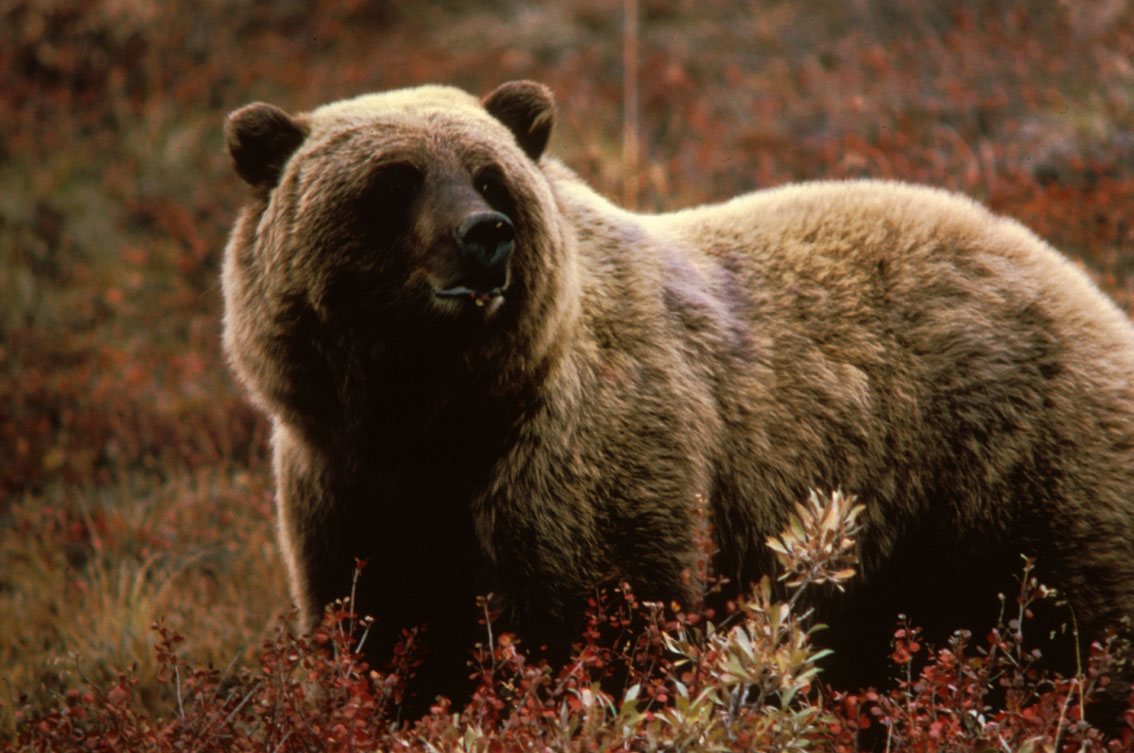
\includegraphics[width=\linewidth]{bear.jpg} % Figure image
% 	\caption{A majestic grizzly bear} % Figure caption
% 	\label{bear} % Label for referencing with \ref{bear}
% \end{figure}

% In hac habitasse platea dictumst. Vivamus eu finibus leo. Donec malesuada dui non sagittis auctor. Aenean condimentum eros metus. Nunc tempus id velit ut tempus. Quisque fermentum, nisl sit amet consectetur ornare, nunc leo luctus leo, vitae mattis odio augue id libero. Mauris quis lectus at ante scelerisque sollicitudin in eu nisi. Nulla elit lacus, ultricies eu erat congue, venenatis semper turpis. Ut nec venenatis velit. Mauris lacinia diam diam, ac egestas neque sodales sed. Curabitur eu diam nulla. Duis nec turpis finibus, commodo diam sed, bibendum erat. Nunc in velit ullamcorper, posuere libero a, mollis mauris. Nulla vehicula quam id tortor ornare blandit. Aenean maximus tempor orci ultrices placerat. Aenean condimentum magna vulputate erat mattis feugiat.

% Quisque lacinia, purus id mattis gravida, sem enim fringilla erat, non dapibus est tellus pellentesque velit. Vivamus pretium sem quis leo placerat, at dignissim ex iaculis. Donec neque tortor, pharetra quis vestibulum id, tempus scelerisque mi. Cras in mattis est. Integer nec lorem rutrum, semper ligula bibendum, iaculis neque. Sed in nunc placerat, viverra dui in, fringilla sem. Sed quis rutrum magna, vitae pellentesque eros.

% Praesent maximus mauris vitae nisl pulvinar, at tristique tortor aliquam. Etiam sit amet nunc in nulla vulputate sollicitudin. Aliquam erat volutpat. Praesent pharetra gravida cursus. Quisque vulputate lacus nunc. Integer orci ex, porttitor quis sapien id, eleifend gravida mi. Etiam efficitur justo eget nulla congue mattis. Duis commodo vel arcu a pretium. Aenean eleifend viverra nisl, nec ornare lacus rutrum in.

% Vivamus pulvinar ac eros eu pellentesque. Duis nibh felis, sagittis sed lacus at, sagittis mattis nisi. Fusce ante dui, tincidunt in scelerisque ut, sagittis at magna. Fusce tincidunt felis et odio tincidunt imperdiet. Cras ut facilisis nisl. Aliquam vitae consequat metus, eget gravida augue. In imperdiet justo quis nulla venenatis accumsan. Aliquam aliquet consectetur tortor, at sollicitudin sapien porta sed. Donec efficitur mauris id rhoncus volutpat. Vestibulum ante ipsum primis in faucibus orci luctus et ultrices posuere cubilia Curae; Sed bibendum purus dapibus tincidunt euismod. Nullam malesuada ultrices lacus, ut tincidunt dolor. Etiam imperdiet quam eget elit tincidunt scelerisque. Curabitur ut ullamcorper dui. Cras gravida porta leo, ut lobortis nisl venenatis pulvinar. Proin non semper nulla.

% Praesent pretium nisl purus, id mollis nibh efficitur sed. Sed sit amet urna leo. Nulla sed imperdiet sem. Donec ut diam tristique, faucibus ligula vel, varius est. In ipsum ligula, elementum vitae velit ac, viverra tincidunt enim. Phasellus gravida diam id nisl interdum maximus. Ut semper, tortor vitae congue pharetra, justo odio commodo urna, vel tempus libero ex et risus. Vivamus commodo felis non venenatis rutrum. Sed pulvinar scelerisque augue in porta. Sed maximus libero nec tellus malesuada elementum. Proin non augue posuere, pellentesque felis viverra, varius urna. Lorem ipsum dolor sit amet, consectetur adipiscing elit. Donec dignissim urna eget diam dictum, eget facilisis libero pulvinar.

% Aliquam ex tellus, hendrerit sed odio sit amet, facilisis elementum enim. Suspendisse potenti. Integer molestie ac augue sit amet fermentum. Vivamus ultrices ante nulla, vitae venenatis ipsum ullamcorper sed. Phasellus gravida felis sapien, ac porta purus pharetra quis. Sed eget augue tellus. Nam vitae hendrerit arcu, id iaculis ipsum. Pellentesque sed magna tortor.

% In ac tempus diam. Sed nec lobortis massa, suscipit accumsan justo. Quisque porttitor, ligula a semper euismod, urna diam dictum sem, sed maximus risus purus sit amet felis. Fusce elementum maximus nisi a mattis. Nulla vitae elit erat. Integer sit amet commodo risus, eget elementum nulla. Donec ultricies erat sit amet sem commodo iaculis. Donec euismod volutpat lacus, ut tempor est lacinia a. Vivamus auctor condimentum tincidunt. Praesent sed finibus urna. Sed pellentesque blandit magna et rhoncus.

% Integer vel turpis nec tellus sodales malesuada a vel odio. Fusce et lectus eu nibh rhoncus tempus vel nec elit. Suspendisse commodo orci velit, lacinia dictum odio accumsan et. Vivamus libero dui, elementum vel nibh non, fermentum venenatis risus. Aliquam sed sapien ac orci sodales tempus a eget dui. Morbi non dictum tortor, quis tincidunt nibh. Proin ut tincidunt odio.

% Pellentesque ac nisi dolor. Pellentesque maximus est arcu, eu scelerisque est rutrum vitae. Mauris ullamcorper vulputate vehicula. Praesent fermentum leo ac velit accumsan consectetur. Aliquam eleifend ex eros, ut lacinia tellus volutpat non. Pellentesque sit amet cursus diam. Maecenas elementum mattis est, in tincidunt ex pretium ac. Integer ultrices nunc rutrum, pretium sapien vitae, lobortis velit.

%------------------------------------------------

\section{Results}

Give the results of your research. Do not, at this stage, try to interpret the results – simply report them. 
This section may include graphs, charts, diagrams etc. (clearly labelled). Be very careful about copyright if you are using published charts, tables, illustrations etc.



%------------------------------------------------

\section{Discussion}

Interpret your findings. What do they show? Were they what you expected? 
Could your research have been done in a better way?


%------------------------------------------------

\section{Conclusion}

These should follow on logically from the Findings and Discussion sections. Summarise the key points of your findings and show whether they prove or disprove your hypothesis. 
If you have been asked to, you can make recommendations arising from your research.

%----------------------------------------------------------------------------------------
%	BIBLIOGRAPHY
%----------------------------------------------------------------------------------------

\printbibliography[title={Bibliography}] % Print the bibliography, section title in curly brackets


%----------------------------------------------------------------------------------------

\end{document}